\documentclass[12pt]{article}
\usepackage[utf8]{inputenc}
\usepackage{hyperref}
\usepackage{listings}
\usepackage{xcolor}
\usepackage{geometry}
\usepackage{graphicx} % For including graphics
\usepackage{minted} % For advanced code listings
\usepackage{listings-solidity}  % Include Solidity highlighting


% Define a custom minted style (optional)
\usemintedstyle{colorful} % You can choose from various styles like 'monokai', 'tango', 'colorful', etc.

% Custom color setup
\definecolor{bashtextcolor}{RGB}{0, 0, 0} % Define black color

% Define a new command for inline code using minted
\newcommand{\codeinline}[1]{\mintinline{text}{#1}}

\geometry{a4paper, margin=1in}

\title{Smart Contracts Exercise 06: \\ Fool the Oracle}
\author{}
\date{}

% Define a new command for inline code with a dark background
\newcommand{\codeblack}[1]{%
  \texttt{\colorbox{black!7}{\textcolor{black}{#1}}}%
}

% Define a new command for inline code with a dark background
\newcommand{\codegrey}[1]{%
  \texttt{\colorbox{black!4}{\textcolor{black}{#1}}}%
}

% Define custom colors (optional)
\definecolor{myURLColor}{RGB}{0, 102, 204} % Example: A shade of blue

\hypersetup{
    colorlinks=true,        % Enable colored links
    linkcolor=blue,         % Color for internal links (e.g., \ref, \cite)
    citecolor=blue,         % Color for citations
    filecolor=magenta,      % Color for file links
    urlcolor=myURLColor     % Color for external URLs
}

% Define a style for code listings
\lstdefinestyle{mystyle}{
    backgroundcolor=\color{lightgray!20},   
    commentstyle=\color{green!50!black},
    keywordstyle=\color{blue},
    numberstyle=\tiny\color{gray},
    stringstyle=\color{red},
    basicstyle=\ttfamily\footnotesize,
    breakatwhitespace=false,         
    breaklines=true,                 
    captionpos=b,                    
    keepspaces=true,                 
    numbers=left,                    
    numbersep=5pt,                  
    showspaces=false,                
    showstringspaces=false,
    showtabs=false,                  
    tabsize=2
}

\lstset{style=mystyle}
% Adding package for header and footer
\usepackage{fancyhdr}
\pagestyle{fancy}

% Define header and footer
\fancyhf{} % Clear current settings
\fancyhead[L]{Smart Contracts 06} % Left header
\fancyhead[R]{\thepage} % Right header with page number

\renewcommand{\headrulewidth}{0.4pt} % Line below header
% \renewcommand{\footrulewidth}{0.4pt} % Line above footer

\begin{document}

\maketitle
\section{Introduction}

Oracles are essential components in decentralized applications that require external data. In this exercise, you will become familiar with synchronous and asynchronous types of oracles, learn about the concept of Decentralized Exchanges (DEXs), and their use as on-chain oracles. Finally, you will practically implement a price oracle manipulation attack using a flash loan.

\subsection*{Prerequisites}

Ensure that you have already installed the following on your system:

\begin{itemize}
    \item \textbf{Node.js} - \url{https://nodejs.org/en/}
    An open-source, cross-platform, back-end JavaScript runtime environment that runs on the V8 engine and executes JavaScript code outside a web browser. 
    \item \textbf{NPM}: Node Package Manager, which comes with Node.js.
\end{itemize}

Open your terminal and run the following commands to verify the installations:

\begin{minted}[bgcolor=gray!5, fontsize=\footnotesize]{bash}
$ node -v
$ npm -v
\end{minted}

Both commands should return the installed version numbers of Node.js and NPM respectively. Node.js provides the runtime environment required to execute JavaScript-based tools like Hardhat, while NPM is used to manage the packages and dependencies needed for development. It is recommended that you use NPM 7 or higher.

% For the purposes of this exercise, you will need an Infura API key and a configured wallet. If you do not have this set up yet, we recommend going through the Smart Contracts Exercise 01: Hello, Blockchain World! where everything is explained. Ensure that configuration variables are set for your Hardhat projects. You can verify this by running:

% \begin{minted}[bgcolor=gray!5, fontsize=\footnotesize]{bash}
% $ npx hardhat vars get INFURA_API_KEY
% $ npx hardhat vars get SEPOLIA_PRIVATE_KEY
% \end{minted}

\subsection*{Project Set Up}

To get started, visit the following \href{https://gitlab.fel.cvut.cz/radovluk/smart-contracts-exercises/-/tree/main/06-Fool-the-Oracle/task/task-code}{GitLab repository} and clone it to your local machine. This repository contains a template in which you will complete this exercise. After you clone the repository, start with the following command within your project folder:

\begin{minted}[bgcolor=gray!5, fontsize=\footnotesize]{bash}
$ npm install
\end{minted}

\section{Oracles}
Smart contracts cannot access data outside the blockchain on their own. They lack HTTP or similar network methods to access external sources. This is intentional to prevent non-deterministic behavior once a function is called. The blockchain does not have an internet connection! However, various Dapp applications often need external information, such as lending platforms, insurance contracts, betting contracts, wrapped cryptocurrencies, synthetics, and others. Whenever a smart contract relies on external data to compute future states, an oracle pattern is required. The disadvantages of oracles include the cost in terms of gas consumption and the risk of dependence on third parties in terms of data manipulation and data availability.

\subsection*{Synchronous Oracles}

In our example, we illustrate a situation where Alice wants to borrow USDC tokens using ETH as collateral. The problem is that the ETH/USDC price is volatile, and we need to know the current price. In a synchronous oracle, external data is periodically pushed into the oracle contract from an oracle controller. The smart contract that needs this external data—in our example, the lending platform—simply trusts that the data in the oracle smart contract is genuine and updated regularly. Look closely at the ilustration in Figure \ref{fig:synchronous-oracles} and the simplified code example below.

\begin{figure}[h!]
  \makebox[\textwidth][ch!]{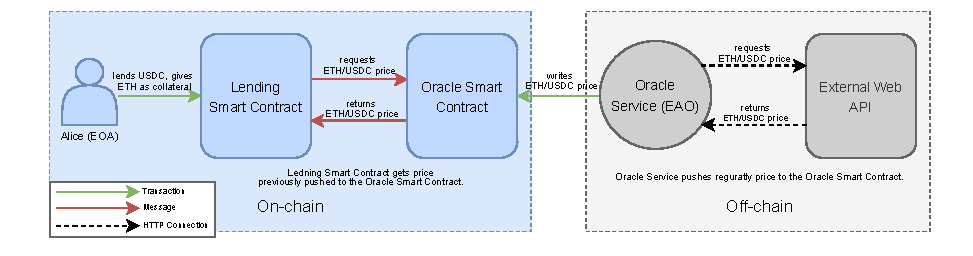
\includegraphics[width=1.1\textwidth]{synchronous_oracle.pdf}}
  \caption{Synchronous Oracles}
  \label{fig:synchronous-oracles}
\end{figure}

% Maybe not needed?
\begin{lstlisting}[language=Solidity]
  contract SimpleSynchronousOracle {
    // Stored ETH/USDC price
    int256 public price;
    // Oracle controller service address
    address public oracleService;
    
    modifier onlyController() {
        require(msg.sender == oracleService, "Not the oracle service");
        _;
    }
    constructor() {
        oracleService = msg.sender;
    }
    // Controller should periodically update the price
    function updatePrice(int256 _price) public onlyController {
        price = _price;
    }
    // Returns the latest price
    function getLatestPrice() public view returns (int256) {
        return price;
    }
}
\end{lstlisting}

\subsection*{Asynchronous Oracles}

An asynchronous oracle provides data in a separate transaction after an initial request. A smart contract requests data from the oracle, which then emits an event. The oracle service fetches the data from an API or another off-chain source and subsequently sends the data back to the contract in a separate transaction.

\begin{figure}[h!]
  \makebox[\textwidth][ch!]{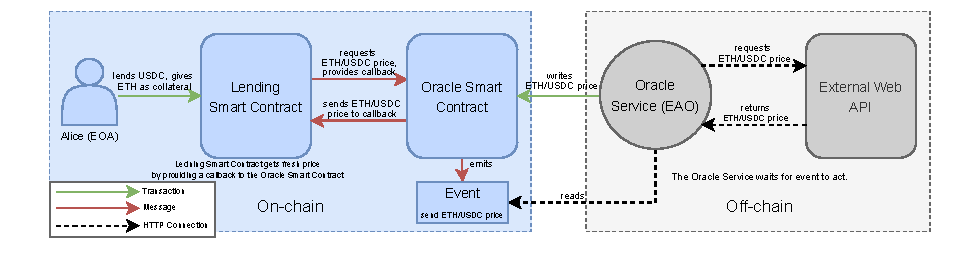
\includegraphics[width=1.1\textwidth]{asynchronous_oracle.pdf}}
  \caption{Asynchronous Oracles}
  \label{fig:asynchronous-oracles}
\end{figure}

To learn more about DEXes and oracles we recommend Berkeley RDI Center on Decentralization \& AI course Decentralized Finance:
\begin{itemize}
\item \href{https://www.youtube.com/playlist?list=PLS01nW3RtgopoR-FHiMwfoMLT-opXlfJF}{DeFi MOOC Lecture 5: DEX}
\item \href{https://www.youtube.com/playlist?list=PLS01nW3Rtgoo70DT2YsBmNUol4134S9C9}{DeFi MOOC Lecture 8: Oracles}
\end{itemize}

\end{document}
